 \begin{center}
 \textbf{
 %\dots
\og 
Notre amour de Dieu face à l’argent
 \fg{}
 %\dots
 }
 \end{center}

Ne croyons pas être si insensibles ou invulnérables face à l’attrait de l’argent. Il fascine comme un faux dieu par toute sorte de chemins : compte en banque, boursicotage, actions, obligations et surtout, jeux d’argent aux gains mirifiques qui ruinent les petits revenus. Et puis, il donne ce sentiment de puissance qui peut tout en achetant tout, parfois même les personnes ! Jésus non seulement nous invite à prendre du recul par rapport aux richesses et à l’argent, mais il est plus radical : il nous dit bien qu’on ne peut servir deux maîtres, si opposés l’un à l’autre. Dieu qui est éternellement fidèle, juste et bon, présent, et MAMON, le trompeur.

\begin{wrapfigure}{l}{1.0cm}
\vspace{-0.4cm}
	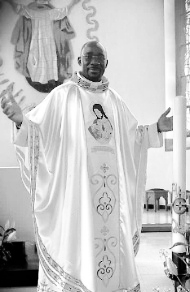
\includegraphics[scale=1.20]{../images/standing_daniel}
\end{wrapfigure}
Que l’argent, certes nécessaire, reste véritablement pour nous un moyen ; que nous en soyons les \og gérants\fg{} responsables qui alimentent, à la manière d’un 
\og gérant avisé\fg{} notre trésor qui se trouve \og dans les tentes éternelles\fg{}. Nous irons certes à contre-courant de l’opinion commune.
Jésus lui aussi a affronté la dérision et, particulièrement, de ceux dont on s’y attendait le moins. Dans l’évangile de ce jour, il dit : \og Gardez-vous de toute avidité, car la vie de quelqu’un, même dans l’abondance, ne dépend pas de ce qu’il possède \fg{}.


\begin{flushright}
Bel été à toutes et à tous !!!
\textit{Père  Daniel  ETTÉ}
\end{flushright}

